\documentclass[11pt,table]{beamer}
\mode<presentation>
\usepackage{etex}
\usepackage{graphicx}
\usepackage{epstopdf}
\usepackage[english]{babel}
\usepackage{tabularx}
\usepackage{booktabs}
\usepackage{mathrsfs}
\usepackage{multicol}
\usepackage{bm}
\usepackage{subcaption}
\usepackage{wrapfig}
\usepackage{dcolumn}
\usepackage{threeparttable}
\usepackage{booktabs}
\usepackage{bbm}
\usepackage{amsmath,dsfont,listings}
\usepackage{amssymb}
\usepackage{rotating}
\usepackage{multirow}
\usepackage{tcolorbox}
\usepackage[authoryear]{natbib}
\usepackage{circledsteps}
\usepackage{qtree}

\usepackage{tikz}
\usetikzlibrary{arrows,decorations.pathmorphing,backgrounds,fit,positioning,shapes.symbols,chains}
\usetikzlibrary{arrows.meta, calc}
\setbeamertemplate{section in toc}[sections numbered]
\setbeamertemplate{caption}[numbered]

\bibliographystyle{Econometrica}

\setbeamersize{text margin right=3.5mm, text margin left=7.5mm}  % text margin
\setbeamersize{sidebar width left=0cm, sidebar width right=0mm}
\setbeamertemplate{sidebar right}{}
\setbeamertemplate{sidebar left}{}

\definecolor{text-grey}{rgb}{0.45, 0.45, 0.45} % grey text on white background
\definecolor{bg-grey}{rgb}{0.66, 0.65, 0.60} % grey background (for white text)
\definecolor{fu-blue}{RGB}{0, 51, 102} % blue text
\definecolor{fu-green}{RGB}{153, 204, 0} % green text
\definecolor{fu-red}{RGB}{204, 0, 0} % red text (used by \alert)
\definecolor{BrewerBlue}{HTML}{377EB8} % Define Brewer Blue
\definecolor{BrewerRed}{HTML}{E41A1C}  % Define Brewer Red
\definecolor{navy}{rgb}{0.0, 0.0, 0.5}

\setbeamertemplate{frametitle}{%
    \vskip-30pt \color{text-grey}\large%
    \begin{minipage}[b][23pt]{\textwidth}%
    \flushleft\insertframetitle%
    \end{minipage}%
}

\setbeamertemplate{navigation symbols}{} 

%%% begin title page
\setbeamertemplate{title page}{
\vskip2pt\hfill
\vskip19pt\hskip3pt

% set the title and the author
\vskip4pt
\parbox[top][1.35cm][c]{11cm}{\LARGE\color{text-grey} \textcolor{red1}{RL}earning:\\[1ex] \inserttitle \\[1ex] \small \quad \\[3ex]}
\vskip17pt
\parbox[top][1.35cm][c]{11cm}{\small Unit 2-1: \insertsubtitle \\[2ex] \insertauthor \\[1ex]}
}
%%% end title page

%%% colors
\usecolortheme{lily}
\setbeamercolor*{normal text}{fg=black,bg=white}
\setbeamercolor*{alerted text}{fg=fu-red}
\setbeamercolor*{example text}{fg=fu-green}
\setbeamercolor*{structure}{fg=fu-blue}

\setbeamercolor*{block title}{fg=white,bg=black!50}
\setbeamercolor*{block title alerted}{fg=white,bg=black!50}
\setbeamercolor*{block title example}{fg=white,bg=black!50}

\setbeamercolor*{block body}{bg=black!10}
\setbeamercolor*{block body alerted}{bg=black!10}
\setbeamercolor*{block body example}{bg=black!10}

\setbeamercolor{bibliography entry author}{fg=fu-blue}
\setbeamercolor{bibliography entry journal}{fg=text-grey}
\setbeamercolor{item}{fg=fu-blue}
\setbeamercolor{navigation symbols}{fg=text-grey,bg=bg-grey}
%%% end colors

%%% headline
\setbeamertemplate{headline}{
\vskip30pt
}
%%% end headline

%%% footline
\newcommand{\footlinetext}{
%\insertshortinstitute, \insertshorttitle, \insertshortdate
}
\setbeamertemplate{footline}{
\vskip2pt
\hfill \raisebox{-1pt}{\usebeamertemplate***{navigation symbols}}
\hfill \insertframenumber\hspace{10pt}
\vskip4pt
}
%%% end footline

%%% settings for listings package
\lstset{extendedchars=true, showstringspaces=false, basicstyle=\footnotesize\sffamily, tabsize=2, breaklines=true, breakindent=10pt, frame=l, columns=fullflexible}
\lstset{language=Java} % this sets the syntax highlighting
\lstset{mathescape=true} % this switches on $...$ substitution in code
% enables UTF-8 in source code:
\lstset{literate={ä}{{\"a}}1 {ö}{{\"o}}1 {ü}{{\"u}}1 {Ä}{{\"A}}1 {Ö}{{\"O}}1 {Ü}{{\"U}}1 {ß}{\ss}1}
%%% end listings

\usepackage{concmath}
\usepackage{xcolor}
\definecolor{red1}{RGB}{206, 17, 38}
\definecolor{blue1}{RGB}{16, 118, 208}
\definecolor{gray1}{RGB}{117, 115, 115}
\usepackage{hyperref}


\newtheorem{proposition}{Proposition}
\newtheorem{assumption}{Definition}

\title[]{Short guides to reinforcement learning}
\subtitle[]{Markov Processes}
\author[D. Rostam-Afschar]{\textcolor{gray1}{Davud Rostam-Afschar (Uni Mannheim)}}
\date[]{\today}
\subject{Econometrics}
\renewcommand{\footlinetext}{\insertshortinstitute, \insertshorttitle, \insertshortdate}
\hypersetup{
    bookmarks=false,
    unicode=false,
    pdftoolbar=false,
    pdffitwindow=true,
    pdftitle={Reinforcement Learning for Business, Economics, and Social Sciences: \insertsubtitle},
    pdfauthor={Davud Rostam-Afschar},
    pdfsubject={Reinforcement Learning},
    pdfkeywords={reinforcement learning, Multi-Armed Bandits},
    pdfnewwindow=true,
}
\def\sym#1{\ifmmode^{#1}\else\(^{#1}\)\fi}

\begin{document}

\begin{frame}[plain]
  \titlepage
\end{frame}

% --------------------------------------------------- Slide --
%\begin{frame}
	%\frametitle{Content}
	%\tableofcontents[]
%\end{frame}

\section{Markov Processes}
{
\setbeamercolor{background canvas}{bg=BrewerBlue}
\begin{frame}
\centering
\Huge
\textcolor{white}{How to predict transitions?}
\thispagestyle{empty}
\end{frame}
}


\section{Markov Chains}
{
\setbeamercolor{background canvas}{bg=BrewerBlue}
\begin{frame}
\centering
\Huge
\textcolor{white}{Markov Chains}
\thispagestyle{empty}
\end{frame}
}


\begin{frame}{Unrolling the Problem}

\begin{center}
\resizebox{0.7\textwidth}{!}{%
\begin{tikzpicture}[node distance=1cm]
\node[fill=lightgray!40!white,rectangle,draw,rounded corners=2pt,inner sep=1ex,line width=1.5pt,minimum height=0.8cm] (O) {\large Agent};
\node[draw,fill=lightgray!40!white,line width=1.5pt, rectangle,rounded corners=2pt,minimum height=1cm,below=of O] (A) {Environment};

%left Path connect
\draw[line width=1.2pt,latex-]  ([yshift=2mm]O.west) -- ++(-3,0) |- ([yshift=-2mm]A.west) node[pos=0.25,left,align=right,font=\scriptsize] { state\\ $S_t$};
\draw[line width=0.7pt,latex-]  ([yshift=-0.5mm]O.west) -- ++(-2.5,0) |- ([yshift=2.5mm]A.west) node[pos=0.25,right,align=left,font=\scriptsize] { reward\\ $R_t$};

%right Path connect
\draw[line width=1.2pt,-latex]  (O.east) -- ++(2.0,0) |- (A.east) node[pos=0.25,right,align=left,font=\scriptsize] {action\\ $A_t$};

\draw[-{Latex[scale=1.5]}] ([yshift=-2mm]A.west) -- ++(-1,0) node[pos=0.4,above=-1pt,font=\scriptsize] {$S_{t+1}$};
\draw[-{Latex[scale=1.2]}] ([yshift=2.5mm]A.west) -- ++(-1,0) node[pos=0.4,above=-1pt,font=\scriptsize] {$R_{t+1}$};


\draw[yshift=-1.9cm,xshift=-2.11cm,line width=1pt,densely dashed] (0,-0.5)--(0,0.5) node[below,pos=0,font=\scriptsize] {next step};
\end{tikzpicture}

}\vspace{3mm}\\
  \small {Goal:} Learn to choose actions that maximize rewards
\end{center}

\end{frame}


\begin{frame}{Unrolling the Problem}

    \begin{itemize}
        \item  Modeling environment dynamics
        \item  Unrolling the control loop leads to a sequence of  states, actions and rewards:
$$
s_0,a_0, r_0, s_1, a_1, r_1, s_2, a_2, r_2,\dots
$$ 

\item  This sequence forms a stochastic process (due to  some uncertainty in the dynamics of the process)

    \end{itemize}

\end{frame}

\begin{frame}{Common Properties}


\begin{itemize}
    \item  Processes are rarely arbitrary
\item They often exhibit some structure
\begin{itemize}
    \item  Laws of the process do not change
\item Short history sufficient to predict future
 

\end{itemize}
\pause
\item  \textbf{Example:} weather prediction

\begin{itemize}
    \item  Same model can be used everyday to predict  weather
\item Weather measurements of past few days sufficient  to predict weather
 
\end{itemize}
\pause

\item  \textbf{Example:} text prediction

\begin{itemize}
    \item  Same model can be used in every conversation to predict next utterance
\item letter sequences of past texts sufficient to predict new sentences
 
\end{itemize}

\end{itemize}
    
\end{frame}


%\begin{frame}{Markov Chains}
    %\begin{itemize}
%\item  Markov invented chains to disprove a colleague’s statement \cite{markov2006}        
        %(that the Law of Large Numbers can only hold for independent sequences of random variables)
%\item He illustrated his new ideas on a vowel/consonant example:
%\item He meticulously listed frequencies of vowel-consonant pairs in the first 20,000 letters of Pushkin’s poem-novel Eugene Onegin
%\item Constructed a transition matrix from this data:
%
    %\end{itemize}
%
%\begin{center}
    %\begin{tabular}{cccc}
    %&&\textit{vowel}&\textit{consonant}\\
%$P=$         & \textit{vowel}&0.175&0.825 \\
         %&\textit{consonant}&0.526&0.474\\ 
    %\end{tabular}
%\end{center}
    %\begin{itemize}
        %\item  He showed that from this matrix one can calculate the average number of vowels and consonants.
%
    %\end{itemize}
%\end{frame}
%
%\begin{frame}{Markov Chains Example}
%
    %\begin{itemize}
        %\item  Construct Markov Chain from frequencies of strings of $k$ letters from the English translation of the novel Eugene Onegin by Pushkin
%
%\item For $k =1,3,5,7$, and then run from a randomly-generated initial condition
%
%\item When $k = 3$, there are English-looking syllables,
%\item When $k =5$ there are English-looking words, and
%\item when $k =7$ the words themselves almost fit together coherently
%
    %\end{itemize}
%
%\vspace{2mm}
    %Example from \citet{hayes2013first}.
%
%\end{frame}
%\begin{frame}{Markov Chains}
%
%\begin{center}
    %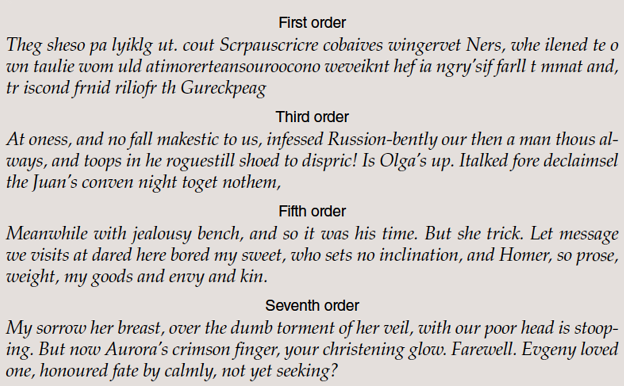
\includegraphics[width=1\textwidth]{figures/11.PNG}
%\end{center}
    %
%\end{frame}
%
%
\section{Markovian and Stationary Processes}
{
\setbeamercolor{background canvas}{bg=BrewerBlue}
\begin{frame}
\centering
\Huge
\textcolor{white}{Markovian and Stationary Processes}
\thispagestyle{empty}
\end{frame}
}


\begin{frame}{Stochastic Process}

\begin{itemize}
    \item  Consider the sequence of states only
\item Definition
\begin{itemize}
    \item  Set of States: $S$
\item Stochastic dynamics: $\mathbb{P}(s_t|s_{t-1}, \dots, s_0)$

\end{itemize}
\vspace{2mm}
\begin{center}
\begin{tikzpicture}[
roundnode/.style={circle, draw=navy, thick, minimum size=7mm}]

% Nodes
\node[roundnode] (circle1) {$S_0$};
\node[roundnode] (circle2) [right=of circle1] {$S_1$};
\node[roundnode] (circle3) [right=of circle2] {$S_2$};
\node[roundnode] (circle4) [right=of circle3] {$S_3$};
\node[roundnode] (circle5) [right=of circle4] {$S_4$};

% Arrows
\draw[-latex, thick] (circle1.east) -- (circle2.west);
\draw[-latex, thick] (circle2.east) -- (circle3.west);
\draw[-latex, thick] (circle3.east) -- (circle4.west);
\draw[-latex, thick] (circle4.east) -- (circle5.west);


% Curved arrow 
\draw[-latex, thick] (circle1) to[bend left] (circle3);
\draw[-latex, thick] (circle2) to[bend left] (circle4);
\draw[-latex, thick] (circle3) to[bend left] (circle5);


\draw[-latex, thick] (circle1) to[bend left=45] (circle4); % Increased bend
\draw[-latex, thick] (circle2) to[bend left=45] (circle5); % Increased bend
\draw[-latex, thick] (circle1) to[bend left=70] (circle5); % Increased bend
\end{tikzpicture}

\end{center}
\end{itemize}
    
\end{frame}

\begin{frame}{Stochastic Process}

\begin{itemize}
    \item  Problem:
\begin{itemize}
    \item  Infinitely large conditional distributions
 
\end{itemize}
\item  Solutions:
\begin{itemize}
\item  \textbf{Stationary process:}\\ \textcolor{red1}{Dynamics do not change over time}\\[2ex]
\item \textbf{Markov assumption:}\\ \textcolor{red1}{Current state depends only on a finite history of past states}\\[2ex]
\item \citet[][Section 15.1]{russell2016artificial}
 
\end{itemize}
\end{itemize}
    
\end{frame}

\begin{frame}{K-Order Markov Process}

\begin{itemize}
    \item  Assumption: last $k$ states sufficient
\pause

\item  First-order Markov Process
\begin{itemize}
    \item  $\mathbb{P}(s_t|s_{t-1},\dots, s_0) = \mathbb{P}(s_t|s_{t-1}$)

 
     
 
\end{itemize}
\begin{tikzpicture}[
roundnode/.style={circle, draw=navy, thick, minimum size=7mm}]

% Nodes
\node[roundnode] (circle1) {$S_0$};
\node[roundnode] (circle2) [right=of circle1] {$S_1$};
\node[roundnode] (circle3) [right=of circle2] {$S_2$};
\node[roundnode] (circle4) [right=of circle3] {$S_3$};
\node[roundnode] (circle5) [right=of circle4] {$S_4$};

% Arrows
\draw[-latex, thick] (circle1.east) -- (circle2.west);
\draw[-latex, thick] (circle2.east) -- (circle3.west);
\draw[-latex, thick] (circle3.east) -- (circle4.west);
\draw[-latex, thick] (circle4.east) -- (circle5.west);

\end{tikzpicture}
\pause
\item  Second-order Markov Process
\begin{itemize}
    \item  $\mathbb{P}(s_t|s_{t-1}, \dots, s_0) = \mathbb{P}(s_t|s_{t-1}, s_{t-2})$
 
\end{itemize}
\begin{tikzpicture}[
roundnode/.style={circle, draw=navy, thick, minimum size=7mm}]

% Nodes
\node[roundnode] (circle1) {$S_0$};
\node[roundnode] (circle2) [right=of circle1] {$S_1$};
\node[roundnode] (circle3) [right=of circle2] {$S_2$};
\node[roundnode] (circle4) [right=of circle3] {$S_3$};
\node[roundnode] (circle5) [right=of circle4] {$S_4$};

% Arrows
\draw[-latex, thick] (circle1.east) -- (circle2.west);
\draw[-latex, thick] (circle2.east) -- (circle3.west);
\draw[-latex, thick] (circle3.east) -- (circle4.west);
\draw[-latex, thick] (circle4.east) -- (circle5.west);


% Curved arrow 
\draw[-latex, thick] (circle1) to[bend left] (circle3);
\draw[-latex, thick] (circle2) to[bend left] (circle4);
\draw[-latex, thick] (circle3) to[bend left] (circle5);

\end{tikzpicture}

\end{itemize}
    
\end{frame}

\begin{frame}{Markov Process}
\vspace{-5mm}
\begin{itemize}
    \item  Commonly, a Markov Process refers to a
\begin{itemize}
     
 \item First-order process

$$
\mathbb{P}\left(s_{t} \mid s_{t-1}, s_{t-2}, \ldots, s_{0}\right)=\mathbb{P}\left(s_{t} \mid s_{t-1}\right) \forall t
$$
\item  Stationary process

$$
\mathbb{P}\left(s_{t} \mid s_{t-1}\right)=\mathbb{P}\left(s_{t^{\prime}} \mid s_{t^{\prime}-1}\right) \forall t^{\prime}
$$
\end{itemize}
\item   \textbf{Advantage:}\\ can specify the entire process with a single concise conditional distribution

$$
\mathbb{P}\left(s^{\prime} \mid s\right)
$$
\end{itemize}
    
\end{frame}


\section{Examples}
{
\setbeamercolor{background canvas}{bg=BrewerBlue}
\begin{frame}
\centering
\Huge
\textcolor{white}{Examples}
\thispagestyle{empty}
\end{frame}
}




\begin{frame}{Examples}
    \begin{columns}[T]
\begin{column}{0.5\textwidth}
\begin{itemize}
    \item  Marrying decision of young women
\begin{itemize}
\item  \textbf{States:}	relationship history
\item \textbf{Dynamics:} age
\end{itemize}

\end{itemize}
\end{column}
\begin{column}{0.45\textwidth}
\centering
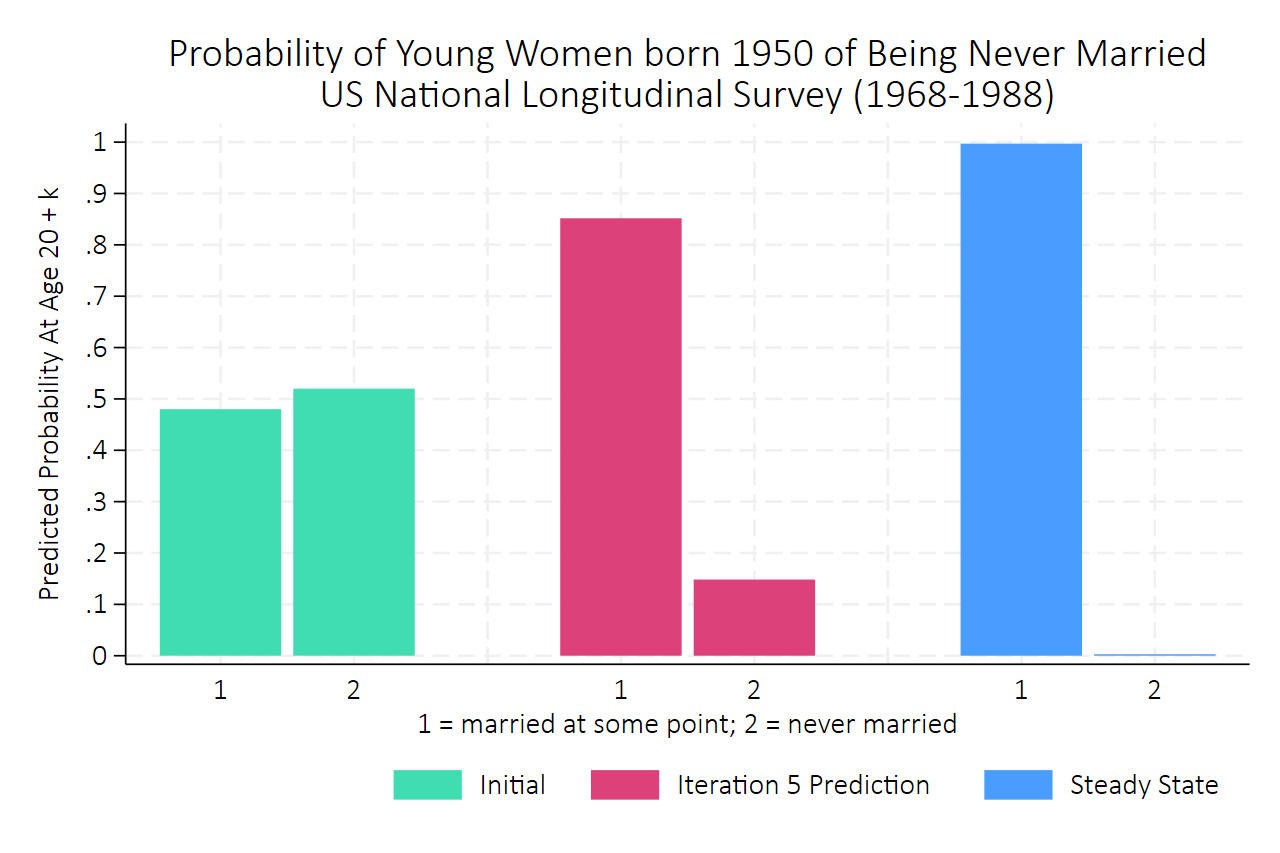
\includegraphics[width=.8\textwidth]{figures/never married.png}
\end{column}
\end{columns}
\pause
    \begin{columns}[T]
\begin{column}{0.5\textwidth}
\begin{itemize}
    \item  Robotic control
\begin{itemize}
\item  \textbf{States:}	$\langle x, y, z,\theta\rangle$
coordinates of joints
\item \textbf{Dynamics:} constant motion
\end{itemize}

\end{itemize}
\end{column}
\begin{column}{0.45\textwidth}
\centering
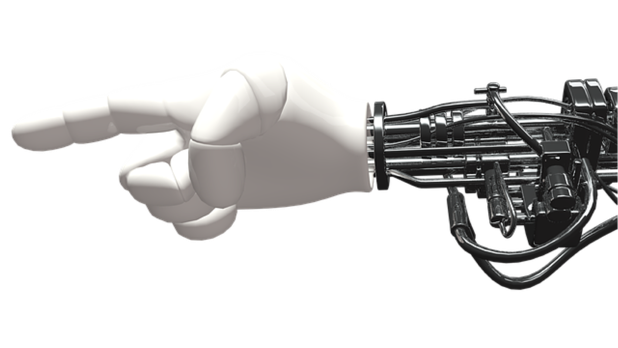
\includegraphics[width=.8\textwidth]{figures/15.png}
\end{column}
\end{columns}
\pause

 \begin{columns}[T]
\begin{column}{0.5\textwidth}
\begin{itemize}
    \item  Inventory management

\begin{itemize}
\item  \textbf{States:} inventory level

\item \textbf{Dynamics:} constant (stochastic) demand

\end{itemize}

\end{itemize}
\end{column}
\begin{column}{0.45\textwidth}
\centering
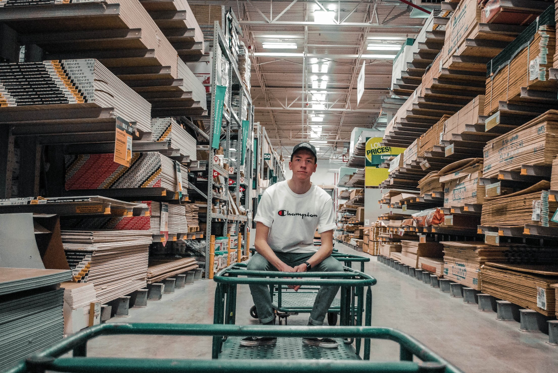
\includegraphics[width=0.8\textwidth]{figures/16.png}
\end{column}
\end{columns}

\end{frame}


\begin{frame}{Inference in Markov Processes}

\begin{itemize}
    \item  Common task is prediction: $\mathbb{P}\left(s_{t+k} \mid s_{t}\right)$


\item  Computation:


$$
\mathbb{P}\left(s_{t+k} \mid s_{t}\right)=\sum s_{t+k} \ldots s_{t+k-1} \prod_{i=1}^{k} \mathbb{P}\left(s_{t+i} \mid s_{t+i-1}\right)
$$

\item Discrete states (matrix operations):
\begin{itemize}
\item  Let $T$ be a $|S| \times|S|$ matrix representing $\mathbb{P}\left(s_{t+k} \mid s_{t}\right)$\\[2ex]
\item  Then $\mathbb{P}\left(s_{t+k} \mid s_{t}\right)=T^{k}$\\[2ex]
\item  Complexity: $\mathcal{O}\left(k|S|^{3}\right)$ 
\end{itemize}
\end{itemize}
    
\end{frame}


\begin{frame}{Example: Marrying as 2-State Markov Process}
\small
Setup: Initial distribution $
p_t = \bigl[\,0.5_{\text{never married}}\;\;0.5_{\text{married}}\,\bigr]
$
\pause
\[
T =
\begin{array}{c|cc}
 & \text{never married} & \text{married} \\ \hline
\text{never married} & 0.5 & 0.5 \\
\text{married}       & 0   & 1
\end{array}\pause
\quad\rightarrow\quad
T^2 =
%\begin{pmatrix}
%0.5^2       & 0.5\cdot0.5 + 0.5\cdot1 \\
%0           & 1
%\end{pmatrix}
%=
\begin{pmatrix}
0.25 & 0.75 \\
0    & 1
\end{pmatrix},...
\]

\pause

Predicted Distributions:
\[
\begin{array}{cc}
\text{Year }k & p_{t+k} = p_{t}\,T^k 
\\\midrule\pause
1 & [\,0.250000\quad 0.750000\,] \\\pause
2 & [\,0.125000\quad 0.875000\,] \\\pause
3 & [\,0.062500\quad 0.937500\,] \\\pause
4 & [\,0.031250\quad 0.968750\,] \\\pause
5 & [\,0.015625\quad 0.984375\,]
\end{array}
\]
\pause
Long Run:
\[
\boldsymbol{\pi} = \lim_{k \to \infty} p_{t+k}
= [\,0\quad 1\,]
\quad(\text{everyone eventually marries})
\]
\end{frame}


%
%\begin{frame}{Example: Marrying as 2-State Markov Process}
%\small
%Setup:
%\[
%T =
%\begin{pmatrix}
%0.8924 & 0.1076 \\
%0 & 1
%\end{pmatrix},
%\quad
%p_t = \begin{bmatrix} 0.3564 & 0.6436 \end{bmatrix}
%\]
%
%\vspace{1em}
%Eigendecomposition:
%\[
%\Lambda = \begin{pmatrix}0.8924 & 0 \\ 0 & 1\end{pmatrix},\quad
%U = \begin{pmatrix}1 & 1 \\ 0 & 1\end{pmatrix},\quad
%U^{-1} = \begin{pmatrix}1 & -1 \\ 0 & 1\end{pmatrix}
%\]
%
%Predicted Distributions (row vector):
%\[
%\begin{array}{cc}
%\text{Step }k & p_{t+k} = p_{t}\,T^k \\ \midrule
%1 & [\,0.3181\quad 0.6819\,] \\
%2 & [\,0.2838\quad 0.7162\,] \\
%3 & [\,0.2533\quad 0.7467\,] \\
%4 & [\,0.2260\quad 0.7740\,] \\
%5 & [\,0.2017\quad 0.7983\,]
%\end{array}
%\]
%
%Long Run:
%\[
%\boldsymbol{\pi} = \lim_{k \to \infty} p_{t+k}
%= [\,0\quad 1\,]
%\]
%
%\end{frame}

\begin{frame}{How Quickly Get Young Women Married?}
\centering
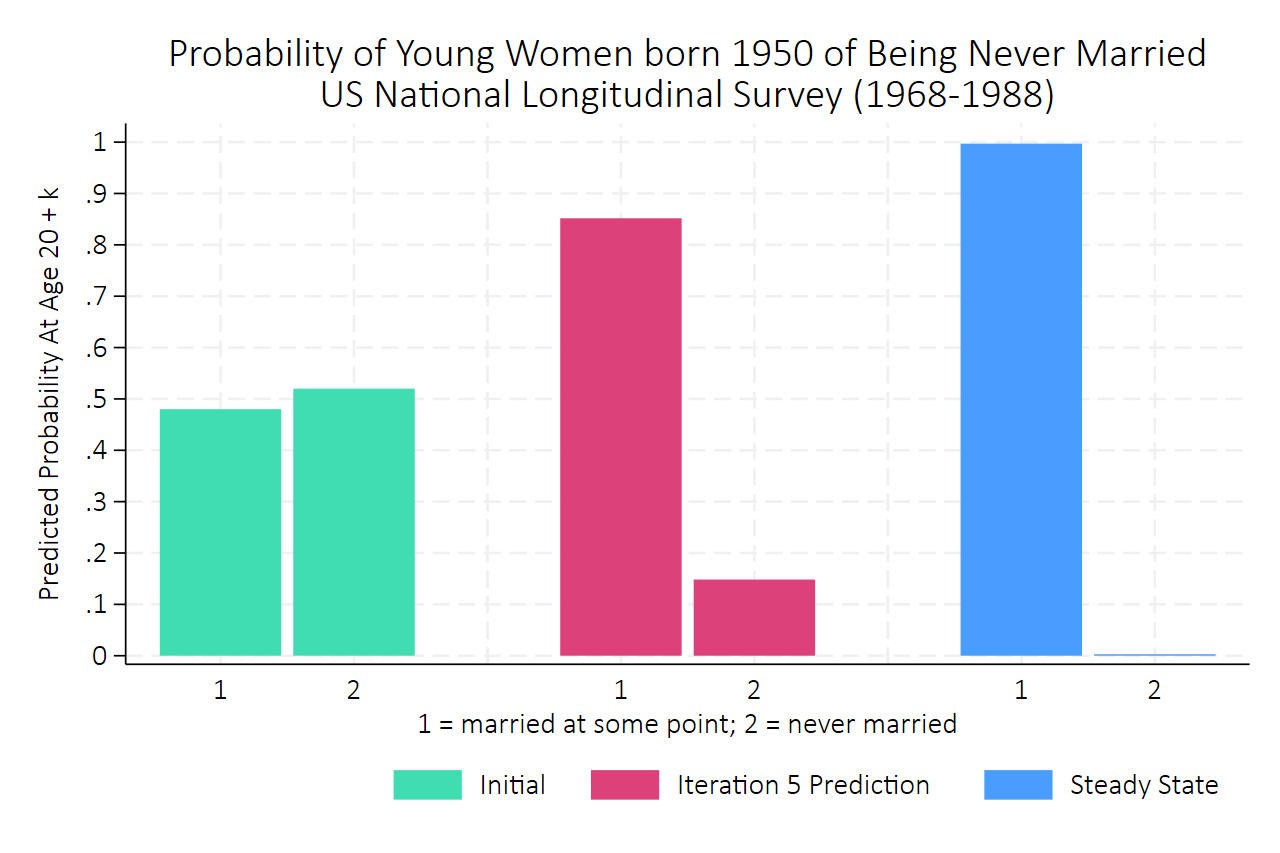
\includegraphics[width=1\textwidth]{figures/never married.png}
\scriptsize
\href{https://rostam-afschar.de/xtsteadystate/xtsteadystate.htm}{\texttt{xtsteadystate nev\_mar if birth\_yr ==50, tw 3dists ini ss pred twowayopt(.)}}
\end{frame}




\begin{frame}{Non-Markovian and/or Non-Stationary Processes}

\begin{itemize}
    \item  What if the process is not Markovian and/or not  stationary?
\item Solution: add new state components until dynamics  are Markovian and stationary\pause
\begin{itemize}
\item Marrying: probability of marrying may depend on: How long a woman has been single, her past relationship history, norms in 1970 vs. 1980
\item Add time since last relationship, number of prior marriages, cohort, ...\pause
 \item Where do we stop?
 
\end{itemize}
%\pause
%\vspace{5mm}

%\begin{itemize}
%\item Robotics: dynamics of $\langle x,y,z,\theta \rangle$ are not stationary when velocity varies...
%\item Solution: add velocity to state description e.g. $\langle x,y,z,\theta,\dot{x},\dot{y},\dot{z},\dot{\theta} \rangle$ 
%\item If acceleration varies... then add acceleration to state
%\item Where do we stop?
 
%\end{itemize}
 
\end{itemize}
    
\end{frame}

\begin{frame}{Markovian Stationary Process}
\vspace{-28mm}
    \begin{itemize}
        \item  \textbf{Problem:} adding components to the state  description to force a process to be Markovian and  stationary may significantly increase computational  complexity

\item \textbf{Solution:} try to find the smallest state description  that is self-sufficient (i.e., Markovian and stationary)

    \end{itemize}
\end{frame}




\begin{frame}{Decision Making}

\begin{itemize}
\item  Predictions by themselves are useless
\item They are only useful when they will influence future  decisions

\item Hence the ultimate task is decision making
\item How can we influence the process to visit desirable  states?

\begin{itemize}
     

\item Model: Markov Decision Process
 \end{itemize}
    \end{itemize}
\end{frame}

\begin{frame}[t,allowframebreaks
]%\nocite{*}
\frametitle{References}
\small
\bibliography{bib}
\end{frame}
\section{Takeaways}
{
\setbeamercolor{background canvas}{bg=BrewerBlue}
\begin{frame}
\centering
\Huge
\textcolor{white}{Takeaways}
\thispagestyle{empty}
\end{frame}
}

\begin{frame}{How Can we Use Markov Processes to Predict Future States?}
\begin{itemize}
    \item Model sequences of states with probabilistic transitions
    \item First-order Markov and stationarity assumptions simplify prediction
    \item Adding state components can restore Markovian/stationary properties---at a computational cost
    \item Prediction relies on transition matrices
    \item Real goal: use predictions for decision-making\\[2ex]
		$\rightarrow$ Markov Decision Processes
\end{itemize}
\end{frame}

\appendix
{
\setbeamercolor{background canvas}{bg=BrewerBlue}
\begin{frame}
\centering
\Huge
\textcolor{white}{Appendix}
\thispagestyle{empty}
\end{frame}
}



\begin{frame}{Prediction and Steady State via Eigendecomposition}

\textbf{Objective:} Predict future state distributions $\mathbb{P}(s_{t+k} \mid s_t)$ and compute the steady-state distribution using eigendecomposition

\vspace{1em}
\textbf{Inputs:}
\begin{itemize}
  \item Initial distribution: $p_t$
  \item Transition matrix: $T$ where $T_{ij} = \mathbb{P}(s_{t+1} = j \mid s_t = i)$
  \item Horizon: $k$ (number of steps ahead)
\end{itemize}

\vspace{1em}
\textbf{Procedure:}
\begin{enumerate}  
  \item Eigendecompose: $T = U \Lambda U^{-1}$
  \item Compute predicted distribution:
  \[
  p_{t+k} = T^k p_t = U \Lambda^k U^{-1} p_t
  \]
  \item Steady state distribution:
  \[
  \boldsymbol{\pi} = \lim_{k \to \infty} p_{t+k}
  \]
\end{enumerate}

\end{frame}


\end{document}
